\section{Method}
Our method is strictly borrowed from Caldarelli et al. \cite{caldarelli2012network}. We investigate the properties of the biased Markov chains formulation of the reflexivity method, in the slightly different context of open collaboration: in this specific context, the bi-partite network has two types of nodes : the editors (i.e., the producing entities) and the articles (i.e. the products). While the method is unchanged, the nature of the input (i.e. the description of the bi-partite network) as well as the interpretation of the relationships are different. Specifically, editors are not competing for the production of an article. They rather cooperate, implicitly according to the rules of peer-production or explicitly through the discussion page attached to each article, in order to increase the quality of the article.

The simplest way to represent a bi-partite network of online collaboration is to consider that an editor is linked to an article when she has ever made a modification. The resulting input of our model is a binary matrix $\mathbf{M}$ of editors and the articles they have modified as shown on Figure \ref{fig:matrix}. 

\begin{figure*}[!t]
\centering
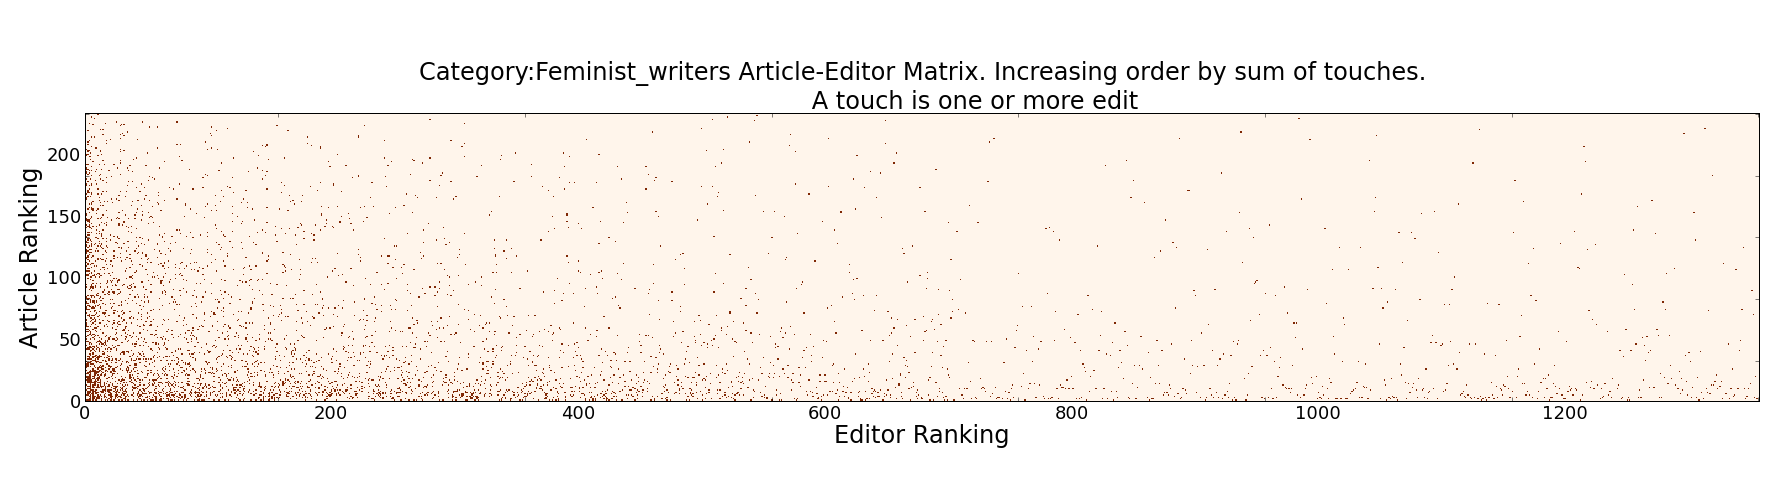
\includegraphics[width=2.0\columnwidth]{Figures/Category_Feminist_writerstriangle_matrix_corrected.png}.
\caption{Typical $\mathbf{M}$ matrix for a Wikipedia category (here, {\it Feminist Writers}) ordered on both dimensions by descending order of number of articles modified by an editor (horizontal axis) and of number editors who have modified an article (vertical axis). The structure of $\mathbf{M}$ is triangular and shows that some editors have a pervasive activity over articles, while most editors edit only a few. Similarly, some articles receive widespread attention by editors, while most articles are modified only by a few editors.}
\label{fig:matrix}
\end{figure*}

<<<<<<< HEAD
\begin{figure*}[!t]
\centering
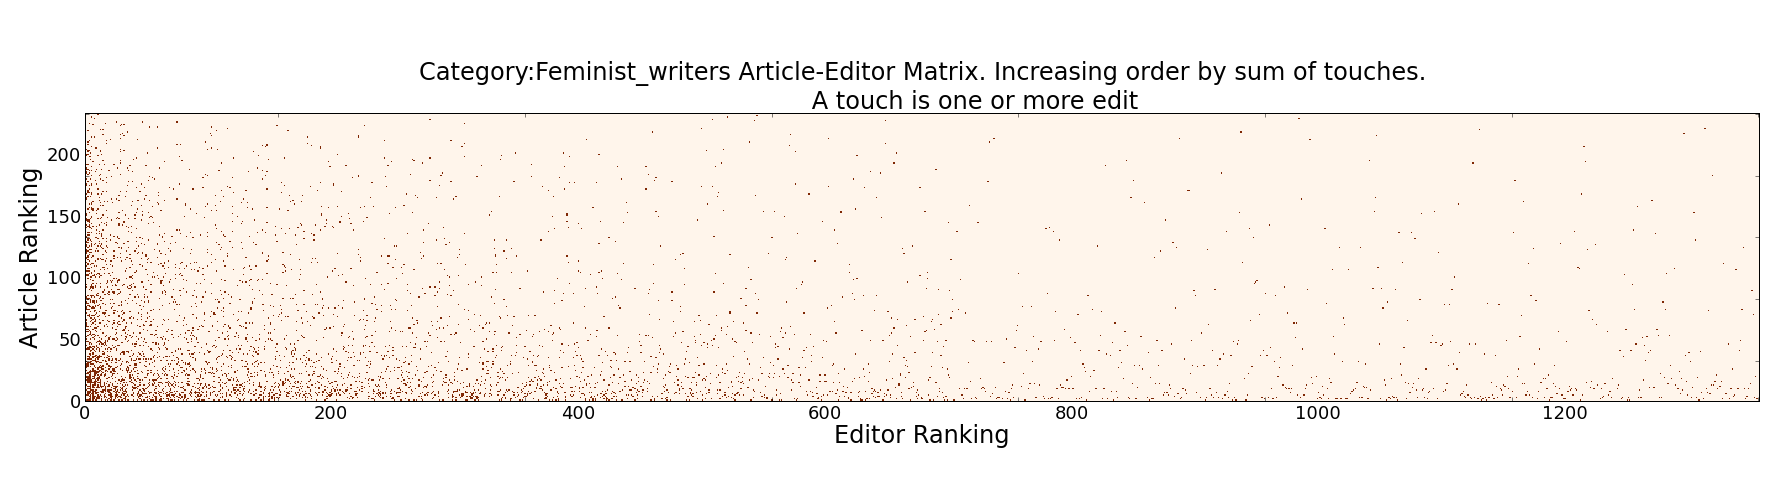
\includegraphics[width=2.0\columnwidth]{Figures/Category_Feminist_writerstriangle_matrix_corrected.png}.
\caption{Typical $\mathbf{M}$ matrix for a Wikipedia category (here, {\it Feminist Writers}) ordered on both dimensions by descending order of number of articles modified by an editor (horizontal axis) and of number editors who have modified an article (vertical axis). The structure of $\mathbf{M}$ is triangular and shows that some editors have a pervasive activity over articles, while most editors edit only a few. Similarly, some articles receive widespread attention by editors, while most articles are modified only by a few editors.}
\label{fig:triangle}
\end{figure*}


The matrix $\mathbf{M}$ shown in Figure \ref{fig:triangle_matrix} shows when an article has changed at some point by a given editor. The matrix is ordered on both dimensions by decreasing order of editors who have changed more articles (vertical axis) and by decreasing order of articles that have been changed by most editors (horizontal axis) for a category of Wikipedia articles (here Feminist Writers). Although it is a rough count, the matrix tells already about the experience of an editor in the given category, and the attention an article has gotten from editors, which is an implicit quality measure according to the second principle of peer-production : peer-review. This count is the zero order of the Article/Editor ranking algorithm, and thus the initiation step is given by 
=======
When ordered on both dimensions by decreasing order of editors who have changed more articles (vertical axis) and by decreasing order of articles that have been changed by most editors (horizontal axis), the matrix $\mathbf{M}$ exhibits a triangular structure, which is at odds with the traditionally accepted idea that editors tend to specialize \cite{}. In that later case, $\mathbf{M}$ should rather be diagonal. On the contrary, some editors have a pervasive activity over all articles, while most editors edit only a few. Similarly, some articles receive widespread attention by editors, while most articles are modified only by a few editors. The matrix $\mathbf{M}$ gives also immediate information on the zero\textsuperscript{th} iteration of the reflexion method: the number of articles modified (horizontal axis) gives information on the expertise of the editor, while the number of editors who have modified an article give an information on the quality of the article : one of the fundamental rules of open source development is that {\it ``Given enough eyeballs, all bugs shallow"} \cite{raymond1999}. The initiation step of the reflexive algorithm is therefore given by,
>>>>>>> sectionized

\begin{equation}
\begin{cases}
 w_{e}^{(0)} = \sum_{a=1}^{N_{a}} \mathbf{M}_{ea} \equiv k_e\\
 w_{a}^{(0)} = \sum_{e=1}^{N_{e}} \mathbf{M}_{ea}  \equiv k_a.\\
\end{cases}
\end{equation}

The principal argument for going to further steps is following : the zero\textsuperscript{th} is quite rough: the number of articles modified tells actually little on expertise of editors because we don't know the value of the modified articles. Similarly the number of editors tells little about the quality of an article because the expertise of the editors who have modified the article is unknown. The second step of the algorithm is therefore the following: if an article has been changed by editors who edited more articles, then the quality of the article should be higher. Similarly, if an editor has edited articles that have been edited by more editors, then the expertise of the editor should be higher {\bf [(the only reason for making this claim is the collaborative nature of Wikipedia, and learning by imitation)]}.  Accordingly, the third step is the following : if an article has been changed by editors who edited more articles, which in turn have been edited by more editors, then the quality of the article should be higher. Similarly, if an editor has edited articles that have been edited by more editors, who in turn have edited more articles, then the expertise of the editor should be higher. The algorithm goes on recursively, incorporating the quality (resp. expertise) information of the article (resp. editor) at the previous step. The way the iterative step was initially formulated is the following, 

\begin{equation}
\begin{cases}
 d_{e}^{(n+1)} = \frac{1}{k_a} \sum_{a=1}^{N_{a}} \mathbf{M}_{ea} \mathbf{w}_{a}^{(n)}\\
 w_{a}^{(n+1)} = \frac{1}{k_e}\sum_{e=1}^{N_{e}} \mathbf{M}_{ea} \mathbf{w}_{e}^{(n)}\\
\end{cases}
\end{equation}

While it is following very well the intuition behind the algorithm, ``The major problem of this formulation is that it is a case of consensus dynamics \cite{shamma2007cooperative}, i.e. the state of a node at iteration t is just the average of the state of its neighbors at iteration t-1". This approach converges rapidly to a fixed point, which is undesirable if the goal is precisely to discriminate between editors and articles as best as possible.

The idea of Caldarelli et al. \cite{caldarelli2012network} is to treat the problem as a problem of a random walker jumping from one node to another along the edges of the bi-partite network. In other words, the random walker jumps with some probability from on editor to a linked article, or from an article to a linked editor. 

We define the weights of vertices to be proportional to the time that an {\it appropriately biased} random walker on the network spends on them in the large time limit \cite{zlatic2010}. We explain a little later why the biases are important. Such weights are the generalization of $k_c$ and $k_p$ and give a measure of competitiveness of countries and of ``dis-quality" of products (here it is quality of articles !!!).


{\bf tell about the stochastic process here} \cite{caldarelli2012network}

{\bf say that it is a ranking algorithm. We care only about the ranking of articles and editors}

The algorithm at step $n$ then writes,

\begin{equation}
\begin{cases}
 w^{(n+1)}_c (\alpha,\beta) = \sum_{p=1}^{N_p}  \mathbf{G}_{cp}(\beta) \mathbf{w}^{(n)}_p (\alpha,\beta)\\
w^{(n+1)}_p (\alpha,\beta) = \sum_{c=1}^{N_c}  \mathbf{G}_{pc}(\beta) \mathbf{w}^{(n)}_c (\alpha,\beta)\\
\end{cases}
\end{equation}

where the Markov transition matrix $\mathbf{\hat{G}}$ is given by 

\begin{equation}
\begin{cases}
\mathbf{G}_{cp}(\beta) = \frac{\mathbf{M}_{cp} \mathbf{k}_{c}^{-\beta}}{\sum_{c' = 1}^{N_c} \mathbf{M}_{c'p} \mathbf{k}_{c'}^{-\beta}}\\
\mathbf{G}_{cp}(\beta) = \frac{\mathbf{M}_{cp} \mathbf{k}_{c}^{-\beta}}{\sum_{c' = 1}^{N_c} \mathbf{M}_{c'p} \mathbf{k}_{c'}^{-\beta}}\\
 \end{cases}
\end{equation}

<<<<<<< HEAD
The random walkers starting from editors jump to articles at odd steps, and back to editors from article at even steps. This is like walking between nodes that are connected by the adjacency matrix \ref{fig:triangle}.



A ranking-by-iteration plot shows how the ranking typically converges over iterations. As shown in Figure \ref{fig:convergence}, the algorithm converges in a non-trivial way, they can be reduced ergodic Markov chains \cite{Firm Grounds}. In the iterative solution we see how certain editors start low, but then climb in rankings. This means that they are editing few articles, but those articles are of higher quality. Likewise certain articles climb over iterations, they are edited by relatively few editors, but those editors are fitter.
=======
where $c'$ and $p'$ are :

Here $G_{cp}$ gives the probability to jump from product p to country c
in a single step, and $G_{pc}$ the probability to jump from country $c$ to
product $p$ also in a single step.


The random walkers starting from editors jump on articles at odd steps, and back on editors from article at even steps. Figure \ref{} shows how the ranking typically converges over iterations. As shown on Figure \ref{fig:convergence}, the algorithm converges in a non-trivial way {\bf (explanation for this?)}. In the iterative solution we see how certain editors start low, but then climb in rankings. This means that they are editing few articles, but those articles are of higher quality. Likewise certain articles climb over iterations, they are edited by relatively few editors, but those editors are fitter.
>>>>>>> sectionized

With the following balance condition,

\begin{equation}
\mathbf{G}_{pc} \mathbf{w}^*_c = \mathbf{G}_{cp} \mathbf{w}^*_p
\end{equation}

An analytical solution can be found \cite{caldarelli}

\begin{equation}
\begin{cases}
 w^*_c = A(\sum^{N_p}_{p=1} M_{cp}k_p^{-\alpha})k_c^{-\beta} \\
w^*_p = B(\sum^{N_c}_{c=1} M_{cp}k_c^{-\beta})k_p^{-\alpha}
\end{cases}
\end{equation}


<<<<<<< HEAD
\begin{figure}[!t]
\centering
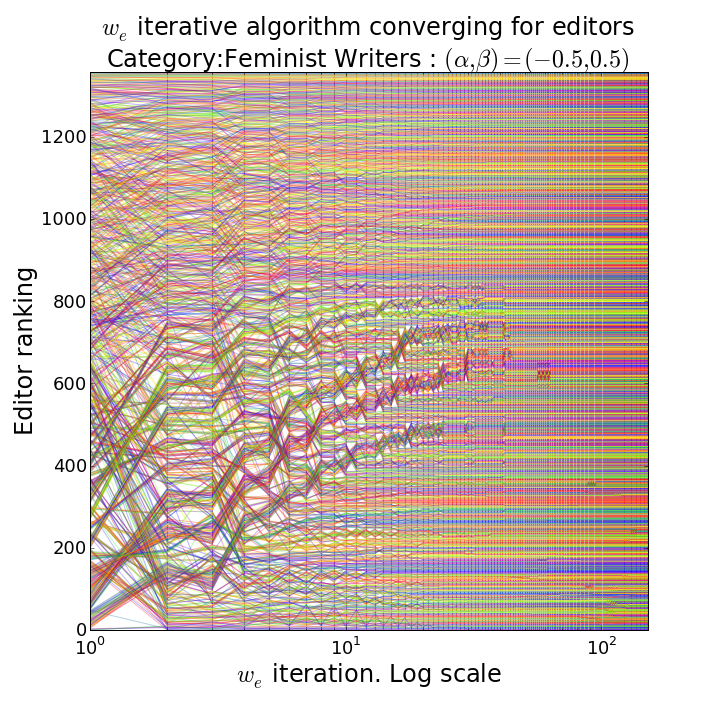
\includegraphics[width=0.9\columnwidth]{Figures/fem_editors_iter_converge.png}.
\caption{Convergence of $w_e$}
\label{fig:convergence}
\end{figure}

that we use onwards. Note that in the case $\alpha = \beta = 0$, the analytical solution is nothing else that the zero$^{th}$..

=======


%\begin{figure}[!t]
%\centering
%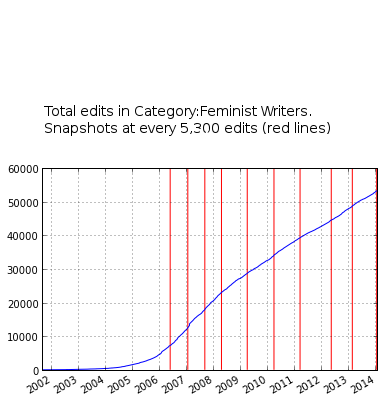
\includegraphics[width=0.9\columnwidth]{Figures/accumulative snapshot points for Feminist Writers.png}
%\caption{Convergence}
%\label{fig:convergence}
%\end{figure}

that we use onwards. Note that in the case $\alpha = \beta = 0$, the analytical solution is nothing else that the zero$^{th}$..

While it relies on the same principles as in \cite{caldarelli2012network}, our proposed model is conceptually different : our ``products" are Wikipedia articles, which are not the basis for competitions but rather for cooperation. Editors enrich the articles together to make best articles. However, like countries, editors have limited capabilities and limited resources (e.g., time), which force them make choices on their contributions.


say the intuition about $\alpha$ and $\beta$.

>>>>>>> sectionized
